\documentclass[conference]{IEEEtran}
\usepackage{amsmath,amsfonts}
\usepackage{algorithmic}
\usepackage{algorithm}
\usepackage{array}
\usepackage[caption=false,font=normalsize,labelfont=sf,textfont=sf]{subfig}
\usepackage{textcomp}
\usepackage{stfloats}
\usepackage{url}
\usepackage{verbatim}
\usepackage{graphicx}
\usepackage{cite}
\hyphenation{op-tical net-works semi-conduc-tor IEEE-Xplore}
% updated with editorial comments 8/9/2021

\begin{document}

\graphicspath{{figures/}} %set folder for figures

\title{Optimizing Open Space for Furniture Layout using Firefly Algorithm and Genetic Algorithm}

\author{
    Randall Fowler and Conor King
}

\maketitle

\begin{abstract}
Abstract goes here...
\end{abstract}

\begin{IEEEkeywords}
Firefly Algorithm, Discrete Optimization, Contour Mapping
\end{IEEEkeywords}

\section{Introduction}
The introduction goes here...

\section{Methodology}
    \subsection{Firefly Algorithm}
    The original FA mimics the behavior of tropical fireflies. Each firefly will represent a solution, and a uniform distribution will be used to initialize the location of each firefly throughout the solution space. This follows a similar method to the particle swarm optimization (PSO) algorithm, but there is a major difference between FA and PSO \cite{swarmIntAlg}. While particles in PSO will move in the direction of a local better solution, fireflies expand upon this by moving toward the current global best solution. Movement toward the global best solution is handled by shifting fireflies toward the brightest firefly with respect to distance.

    The FA is designed for continuous optimization with a maximization objective defined as 
    \begin{equation}
    \label{OptObj}
        Maximize\;\: f(x), x \in \mathbb{R}^D.
    \end{equation}
    It is an unconstrained problem that requires constraints to be added during movement of the fireflies. For a discrete optimization problem, such as the problem described in this paper, new solutions formed after movement can be quantized to integer values.

    Movement of these fireflies is defined by an equation that weights distance similar to absorption of light intensity. Calculation of movement is defined as 
    \begin{equation}
    \label{FireflyMovement}
        x^{t+1}_i = x^t_i + \beta_0 e^{-\gamma r^2_{i,j}} (x^t_j - x^t_i) + \alpha \epsilon^t_i,
    \end{equation}
    where $x^t_i$ represents the location of the $i$th firefly in the $t$th iteration. While the distance between fireflies is a main component in the equation, the weighting is known as the attractiveness. Hyperparameters for this attractiveness term would be $\beta_0$, the attractiveness at zero distance, and $\gamma$, the absorption coefficient. Distance between solutions is calculated using Cartesian distances, and $r_{i,j}$ would be 
    \begin{equation}
    \label{CartesianDistance}
        r_{i,j} = \sqrt{\sum_{k=1}^{D} (x_{i,k} - x_{j,k})^2},
    \end{equation}
    an $l2$ norm of the two fireflies. This attractiveness term will reduce movement between fireflies if the distance is relatively large, and this will enable movement toward the global best solution while encouraging more movement toward local bests.

    The final term in the movement equation \ref{FireflyMovement} represents the exploration or noisy movement of the fireflies. While the vector $\epsilon^t_i$ will contain random numbers following a normal distribution with zero mean and unity variance, the hyperparameter $\alpha$ will be a scaling factor. Both $\beta_0$ and $\alpha$ will depend greatly on the scaling of the solution vector.

    Another parameter in FA would be the time allowed for movement. With FA being a search algorithm to reduce the need for exhaustive searching. Algorithm \ref{FireflyAlgorithm} describes the pseudocode for FA. For the specified amount of time, the algorithm will iterate over all fireflies, check if the value of other fireflies is greater, and move if so. After every firefly has been visited, the known best will be saved.

    \begin{algorithm}
    \caption{Firefly Algorithm}
    \label{FireflyAlgorithm}
    \begin{algorithmic}
    \STATE Initialize fireflies $x_i, i = 1, 2, ..., N$.
    \STATE Evaluate the objective function $f(x_i)$ for each firefly.
    \STATE Set time $t = 0$.
    \WHILE{$t < T$}
        \FOR{$i = 1$ to $N$}
            \FOR{$j = 1$ to $N$}
                \IF{$f(x_j) > f(x_i)$}
                    \STATE Move firefly $i$ toward $j$ using equation \ref{FireflyMovement}.
                    \STATE Evaluate the objective function $f(x_i)$.
                \ENDIF
            \ENDFOR
        \ENDFOR
        \STATE Sort fireflies by objective function and update the best solution.
        \STATE $t = t + 1$.
    \ENDWHILE
    \end{algorithmic}
    \end{algorithm}

    \subsection{Defining Objects in the Room}
    To reduce the complexity of objects shape, location, and orientation, the optimization of the room layout is defined as a discrete problem with rectangular objects. Each object will have a width, depth, rotation, reserved space, and a unique identification (uid). Rotation is defined by an enumeration of up, right, down, and left with values of 0, 1, 2, and 3 respectively. For values larger or smaller than the enumerated values, the value will be shifted to the respective values, 4 would be equivalent to 0, and -1 would be equivalent to 3. The names of the enumeration can be interchangeable with north, east, south, and west. Reserve space will be considered to be the space in front of the object from wherever it is facing. When something is facing up, the reserve space of the object will be above the object.
    
    Width and depth are the size parameters defining the size by orientation. If an object is facing up or down, the width will represent the distance in the x direction while depth would be in the y direction. This will be the opposite case for facing left and right as depth will be in the x direction and width will be in the y direction. Reserve space will be the distance in front of the object that is reserved open space, and the width of the reserved space will be the same as the width of the object. The purpose of the reserved space is to allow access to the object; most objects, such as a desk, door, or bookshelf, would require space in front of it for someone to stand or sit. Objects that need reserved space in more than one direction are not considered in this paper, but it wouldn’t be a large change to add it.
    
    For the uid, objects will have an identification equal to a prime number larger than 1. The reason for this is due to the nature of solving conflicts when moving objects. An open space would be given a value of 1 and adding an object would be to multiply the rectangular area by its uid. If a point in the graph has a non-prime number, this will be an indication of an overlap between objects.
    

    \subsection{Defining the Room}
    A room will be defined simply as its width, height, and graph. The graph will be defined as an array with relative units shared between the sizing of the objects and room. This graph will hold the value 1 for being an open space and a value larger than one is an object taking up that space. For the uid graph, the reserved space will be included in the graph, but for open space graph, the reserved space will not be included. Since reserved space will be open, it will be considered for the evaluation of the layout.

    \subsection{Solution Vector}
    Initialization of fireflies requires a uniform distribution amongst the solution space. Each firefly will have an associated solution vector holding the location and rotation of every object in the room. 
    
    The dimensions of the solution vector will be defined by the number of objects in the room, and the order of these objects will be by shape and distance from a reference point. This reference point is chosen to be the origin, bottom left corner of the room. One issue that arises from having a set index for the solution vector is that multiple solutions could be the same due to objects having the same shape. This shape is defined by its width, depth, and reserved space. Indexing of the solution vector will be iterated by the different shapes, and for each shape, there will be an indexing in the order of distance to the origin.
    
    Some objects, such as doors and windows, are not moveable or rotatable in the room. For these objects and others that may not want to be moved, these will be left out of the solution vector. However, if a shape is moveable, but not rotatable, it will be included in the solution vector without a rotation variable and as its own shape. Any additional objects with the same shape and without rotation will be grouped together in the solution vector, similar to shapes with rotation.
    
    Random placement of objects within the room will be bound to the size of the room. Coordinates and rotation will be gathered from a uniform distribution, and if the object does not fit in the room, a new coordinate and rotation will be gathered. This technique for generating initial solutions may require more time for more objects as objects will often fail when fitting.
    

\section{Design Decisions}
    \subsection{Objective Function}
    The purpose of this project is to design an optimal layout for a room with known objects. However, this is a challenging problem to address as optimizing the layout of a room is biased toward the opinion of the user. A common preference for individuals when designing their room is to have the largest amount of open space possible. With a set number of objects, the amount of open space would be the same for every possible room arrangement, but maximizing open space for this project holds a different definition. The objective of maximizing open space consists of maximizing the roundness of open areas. This means that larger open spaces would be preferred, but stretched open space would be less preferable than more circular open spaces; A large rectangular open space would be preferred over a long rectangle with the same area.
    
    At first, this objective function was thought to be its own optimization problem where largest ratio of area to perimeter would be useful for estimating value of the room. However, another method emerged to try and satisfy the objective function. A pseudo contour map of the room could be created to find the distance between objects and maximize on spreading objects around the room. For less objects, the optimal solution could be to push everything against the walls, but for a larger number of objects, the layout would need to be creative about placement.
    
    A contour map for the room would be an estimate of distance between objects at every point in the room. Objects themselves would have a value of 0 since that is the location of an object, and the walls could be either seen as an object or not. For this project, it was decided to treat the walls as an object, but exploring the other option could be insightful.
    
    The first idea of a contour map thought of would be known as open distance, and this represents the product of width and height of the open space at a given position of the graph. This algorithm is simply created by iterating over all positions of the graph and getting the width by moving up and down till hitting a wall or object, and the height similarly with left and right. Results for this method are shown in figure \ref{open_dist_fig}, and it is difficult to spot where the objects actually are. 
    \begin{figure}
        \centering
        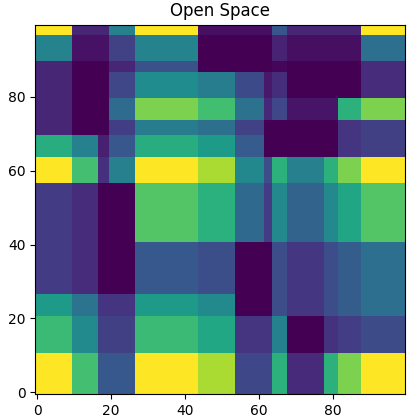
\includegraphics[width=0.3\textwidth]{contour_map_opendist.png}
        \caption{Open Distance Contour Map}
        \label{open_dist_fig}
    \end{figure}

    The second idea of a contour map was to use Euclidean distance to the nearest object or wall. This algorithm would require a good search method that could keep its searching distance to under the distance to the nearest wall. However, Taxicab geometric distance would provide a similar contour map, but the algorithm could be greatly improved. 

    Algorithm \ref{taxicab_eval} shows the method for calculating distances. All points would be initialized as a number larger than possible, objects would be added as 0 values, and the search would begin by adding all nodes with 0 value to a list of nodes. While there are nodes in the list, each node will be iterated through, and if a neighbor has a larger value than the current node, the neighbor will be given a value of one larger than its own. After iterating through all nodes, it will then add all nodes with a value of one larger than the nodes it just visited. Eventually, all points in the map will have a distance. Results of this algorithm can be seen in figure \ref{taxicab_dist_fig}.

    \begin{algorithm}
        \caption{Taxicab Distance Contour Map}
        \label{taxicab_eval}
        \begin{algorithmic}
        \STATE Initialize map to height or width of room.
        \STATE Add all objects as 0 values.
        \STATE Add all 0 value nodes to a list of nodes.
        \WHILE{There are nodes in the list}
            \FOR{Each node in the list}
                \FOR{Each neighbor of the node}
                    \IF{Neighbor has a larger value than the current node}
                        \STATE Neighbor is given a value of one larger than the current node.
                    \ENDIF
                \ENDFOR
            \ENDFOR
            \STATE Add all nodes with a value of one larger than the nodes it just visited to the list.
        \ENDWHILE
        \end{algorithmic}
    \end{algorithm}

    \begin{figure}
        \centering
        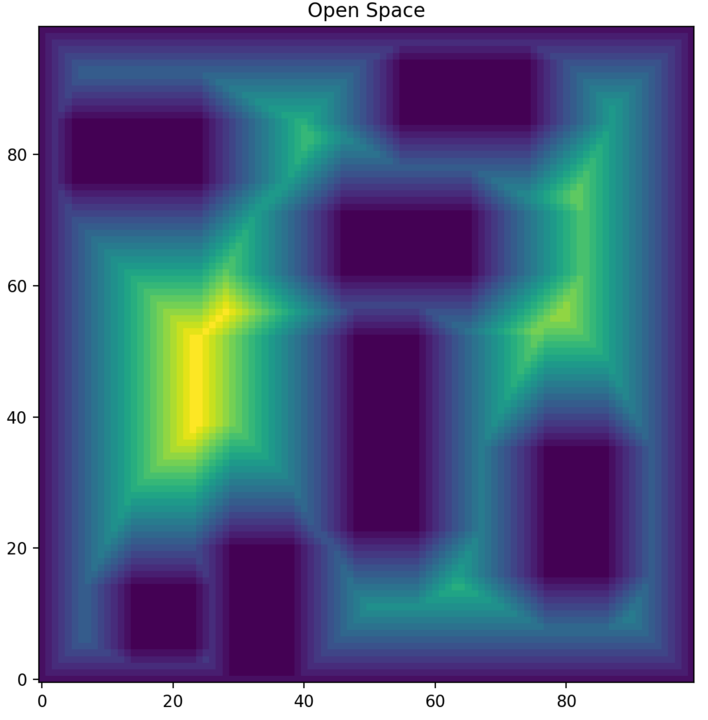
\includegraphics[width=0.3\textwidth]{contour_map_taxicab.png}
        \caption{Taxicab Distance Contour Map}
        \label{taxicab_dist_fig}
    \end{figure}

    Once the contour map has been found, evaluation of the map will provide the objective function. This value can be found by summing the entire contour map. Larger values will be calculated if there is more space between objects, and the calculated values could be normalized using the size of the room.
    

    \subsection{Types of Conflicts}
    Hello, types of conflicts go here...

    \subsection{Noise Seperation}


    \subsection{Hyperparameters}
    

\section{Experimental Tests}
Experimental tests go here...

\section{Conclusions}
Conclusions go here...

\section*{Acknowledgment}
Thankful for...

\begin{thebibliography}{1}
    \bibliographystyle{IEEEtran}
    
    \bibitem{swarmIntAlg}
    Slowik, A. (Ed.). (2020). Swarm Intelligence Algorithms: A Tutorial (1st ed.). CRC Press. https://doi.org/10.1201/9780429422614
    
    \bibitem{ref2}
    Reference 2 goes here...
    
\end{thebibliography}

\end{document}


